\section*{Problemas PI:}

Para os problemas apresentados, realizar:
\begin{enumerate}[label=\alph*)]
    \item Simulação usando MATLAB/Simulink realizando análise dos resultados com relação a estabilidade e 
    resposta dinâmica do sistema
    \item Analisar o LGR sem/com controlador
    \item Determine o tempo de amostragem e realize a discretização dos controladores. Comparar com a
    solução continua.
    \item Discretizar os sistemas (controlador e planta) e analisar a estabilidade usando o método de Jury e
    Routh Hurwitz.
\end{enumerate}
    

\subsection*{Problema 1:}

Para esse problema, o modelo de um motor possui como FT a equação \ref{eq:Gp1}. 

\begin{equation}
    G_p = \frac{4}{s^3+3s^2+10s}
    \label{eq:Gp1}
\end{equation}

A FT de MF, com um controlador proporcional é o visto na equação \ref{eq:Gmf1}.

\begin{equation}
    G_{mf} = \frac{4kp}{s^3+3s^2+10s + 4kp}
    \label{eq:Gmf1}
\end{equation}

Foi visto no desenvolvimento da questão que para o sistema ser estável o ganho propocional deve estar
no intervalo: $0<kp<7,5$. Escolheu-se ter um pólo em -2 e por isso foi determinado $kp = 4$.


\subsubsection*{a)}
    A estabilidade do sistema foi verificada através de uma entrada ao degrau. Pelo desenvolvimento analítico,
    o erro em regime estacionário deve ser zero a uma entrada ao degrau, espera-se obter o mesmo resultado
    pela simulação no MATLAB através do Código \ref{Q1A}.

    \begin{lstlisting}[language=Matlab,label=Q1A,caption=Análise da estabilidade]
%FT sem controlador
num = 4;
den = [1 3 10 0];
G = tf(num,den);
%FT com controlador
kp = 4;
Gmf = tf(kp*num,[1 3 8 4*kp]);

% a)
[y,t] = step(Gmf);
figure
plot(t, y, 'LineWidth', 2);
legend('c(t)')
grid
    \end{lstlisting}

    A Figura \ref{fig:Q1A} apresenta a resposta do sistema ao degrau.


    \begin{figure}[!ht]
        \centering
        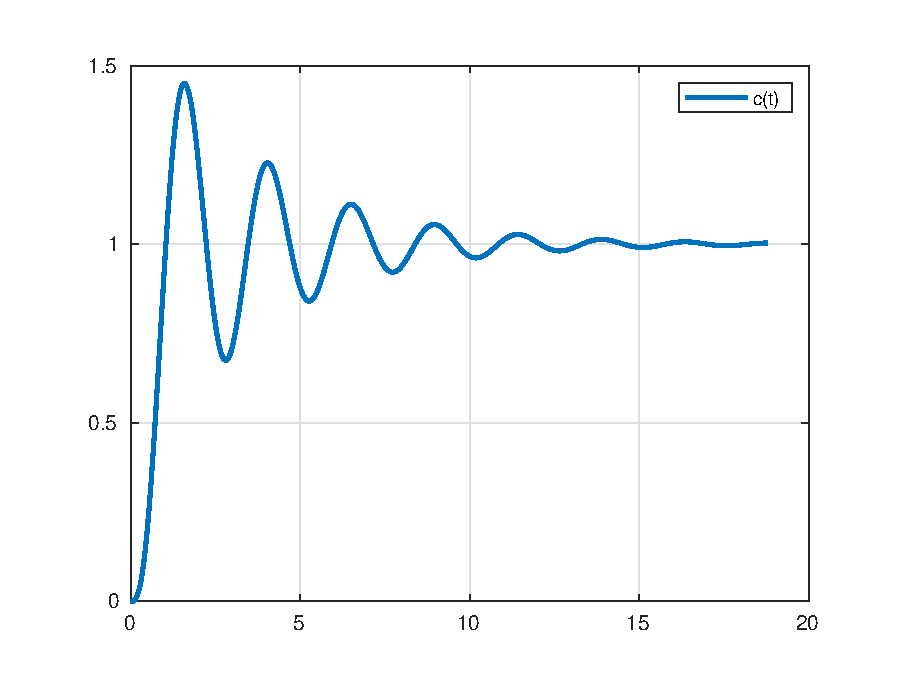
\includegraphics[width = 0.75\linewidth]{Figuras/ProblemasPI/Problema1/step1.eps}
        \caption{Gráfico da resposta ao degrau do sistema}
        \label{fig:Q1A}                   
    \end{figure}

    Podemos verificar que o erro em regime estacionário do sistema tende a zero, assim como determinado 
    através do cálculo analítico. Ainda, podemos verificar que o sistema utilizando um controlador proporcional
    mantém a existência de um sobrevalor percentual.

    Através do \mcode{stepinfo} verifica-se que o sobrevalor percentual é precisamente de 44,93\% e o tempo
    de subida de $T_r =0,6 \text{ s} $. 

\subsubsection*{b)}

    Como já feito anteriormente na avaliação, através da função \mcode{rlocus} é possível traçar o LGR 
    do sistema. A Figura \ref{fig:LGR1Bsem} é o LGR do sistema sem o controlador. Pode-se verificar que
    o sistema possui três pólos, com um deles na origem e os outros dois, um par complexo. Como estão 
    no semiplano esquerdo o sistema é estável à resposta ao degrau. Porém o pólo no zero torna o sistema
    mais lento.
    

    \begin{figure}[!ht]
        \centering
        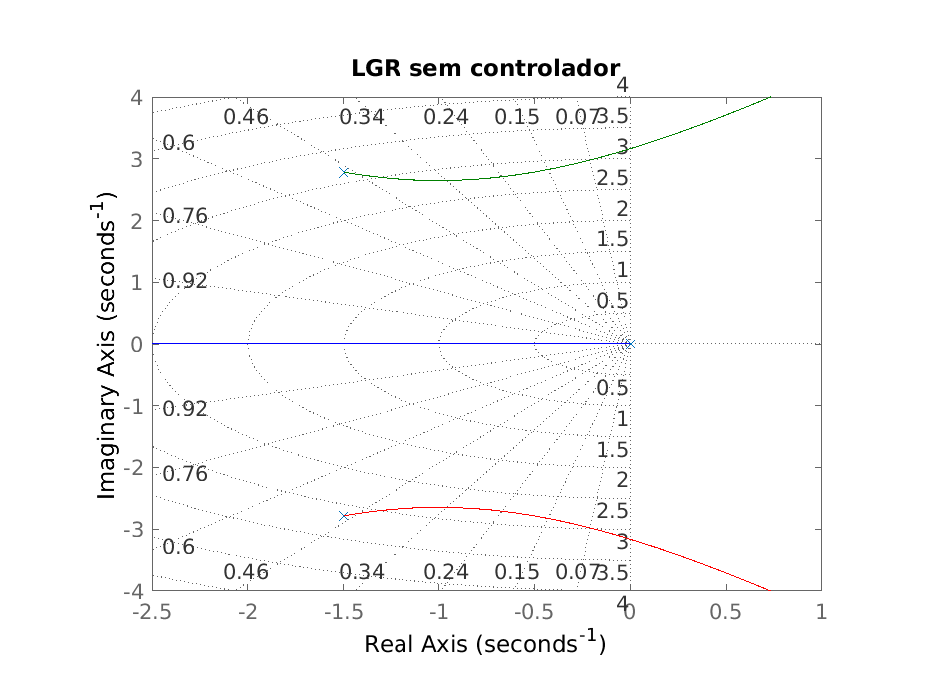
\includegraphics[width = 0.75\linewidth]{Figuras/ProblemasPI/Problema1/LGRsemControlador.eps}
        \caption{Lugar geométrico das raízes sem controlador}
        \label{fig:LGR1Bsem}                   
    \end{figure}

    O objetivo do controlador proporcional foi colocar um pólo em -2. Pelo LGR do sistema em MA, o pólo do zero
    é o único que ao variar o ganho se desloca sobre o eixo real. Pode-se verificar através da Figura  
    \ref{fig:LGR1Bcom} que o objetivo foi alcançado.

    \begin{figure}[!ht]
        \centering
        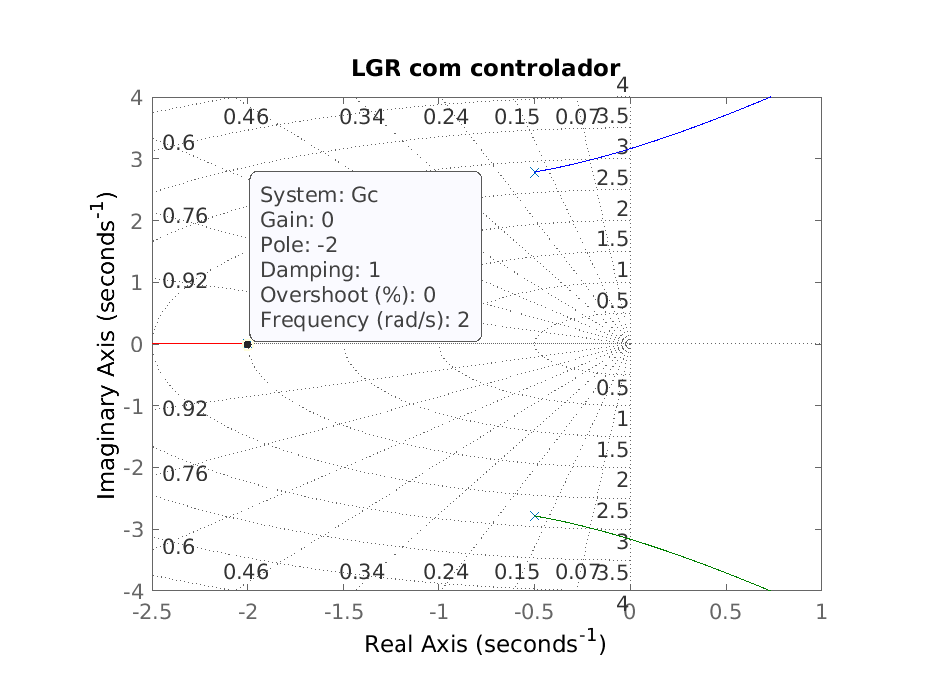
\includegraphics[width = 0.75\linewidth]{Figuras/ProblemasPI/Problema1/LGRcomControlador.eps}
        \caption{Lugar geométrico das raízes com controlador}
        \label{fig:LGR1Bcom}                   
    \end{figure}

    \newpage    
    \subsubsection*{c)}

        Como anteriormente, o tempo de amostragem foi determinado pelo tempo de subida divido por dez. 
        O sistema foi discretizado utilizando o segurador de ordem zero (ZoH). O Código \ref{Q1C} apresenta
        a discretização do modelo e a criação do gráfico da resposta do sistema a entrada degrau.

        \begin{lstlisting}[language=Matlab,label=Q1C,caption=Análise da estabilidade]
    Ts = stepinfo(Gmf).RiseTime/10; %Tr = 0.6000
    Gmfz = c2d(Gmf,Ts, 'zoh');
    [yz,tz] = step(Gmfz); %salvando resultado do step

    figure %fazendo uma figura para comparar
    plot(t, y, 'LineWidth', 2)
    hold on
    stairs(tz, yz, 'LineWidth', 2);
    hold off
    legend('c(t)', 'c(kT)')
    grid

    %utilizando MAPE para avaliacao numerica
    ape = abs((yz - y(1:length(yz)))/y(1:length(yz))); 
    mape = mean(ape(isfinite(ape))); %retira o erro percentual do y=0
    %mape = 3.2708e-04
        \end{lstlisting}

    O tempo de amostragem obtido foi de 60 ms. O MAPE foi de $3,27 \cdot 10^{-2}$ \%.
    A FT em MF disceta é apresentada na equação \ref{eq:Gmfz1}.
    A Figura \ref{fig:Stepctds1} apresenta a resposta dos sistema contínuo e discretizado sobrepostos. 

    \begin{equation}
        G_{mf}(z) = \frac{0.0005503 z^2 + 0.002103 z + 0.0005029}{z^3 - 2.807 z^2 + 2.646 z - 0.8353}
        \label{eq:Gmfz1}
    \end{equation}


    \begin{figure}[!ht]
        \centering
        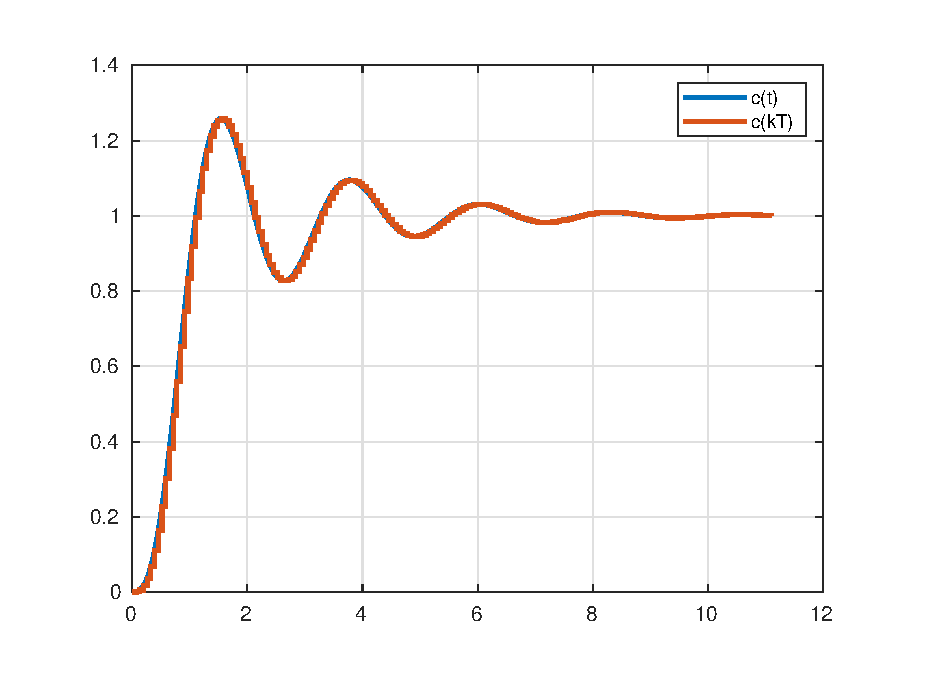
\includegraphics[width = 0.75\linewidth]{Figuras/ProblemasPI/Problema1/resposta_ao_degrau.eps}
        \caption{Resposta ao degrau}
        \label{fig:Stepctds1}                   
    \end{figure}

    Visualmente o sistema discreto se aproxima da resposta contínua. Porém, como vem sendo feito nessa 
    avaliação, verificamos a qualidade da discretização através do MAPE. Para essa discretização o 
    MAPE foi de $3,27 \cdot 10^{-2}$ \%. Um baixo valor de erro.

\subsubsection*{d)}

O polinômio característico do sistema contínuo pode ser visto na equação \ref{eq:pcsc1}. O método
de Routh consiste em verificar se há mudança de sinal na primeira coluna da tabela, se não ocorre
o sistema será estável, se ocorrer, instável. A Tabela \ref{tab:RE1} apresenta o desenvolvimento do
resultado obtido 

\begin{equation}
    Q(s) = s^3+3s^2+10s+16
    \label{eq:pcsc1}
\end{equation}

\begin{table}[!ht]
    \centering
    \vspace{0.5cm}
    \caption{Análise de estabilidade pelo método de Routh} 
    \begin{tabular}{r|lr}
        
        1 & 1 & 10 \\
        2 & 3 & 16 \\
        3 & 4{,}67\\
    \end{tabular}                
    \label{tab:RE1}
\end{table}

Verificamos que o sistema contínuo é estável.

O polinômio característico do sistema discreto pode ser visto na equação \ref{eq:pcsd1}.

\begin{equation}
    Q(z) = z^3 - 2.807 z^2 + 2.646 z - 0.8353
    \label{eq:pcsd1}
\end{equation}

A Tabela \ref{tab:JE1} apresenta o desenvolvimento do método de Jury para esse sistema.

\begin{table}[!ht]
    \centering
    \caption{Análise de estabilidade} 
    \begin{tabular}{l| r r r r}
         & $z^0$ & $z^1$ & $z^2$ & $z^3$\\
        \hline
        1 & -0{,}8353 & 2{,}646 & -2{,}807 & 1\\
        2 & 1 & -2{,}807 & 2{,}646 & -0{,}8353\\
        3 & -0{,}3013 & 0{,}5968 & -0{,}3023 & 0\\
    \end{tabular}                
    \label{tab:JE1}
\end{table}

Para verificar a estabilidade, como nosso polinômio é de ordem 3, devemos conferir os 4 critérios.

- O primeiro critério: $Q(1)= 3,7 \cdot 10^{-3} > 0$, satisfeito; \\
- O segundo critério: $-1^3 Q(-1) = 7,2883 > 0$, satisfeito;\\
- O terceiro critério: $|a_0| = 0,8353 < 1 = |a_3|$, satisfeito; \\
- O quarto critério: $|b_0| = 0,3023 > 0,3013 = |b_3| $, satisfeito. 

Como o sistema discreto atende os quatro critérios de Jury necessários, é um sistema estável.

\subsection*{Problema 2:}

    A FT da planta é vista na equação \ref{eq:Gp2}. 

    \begin{equation}
        G_p = \frac{1}{(2.105s+1)(0.095s+1)}
        \label{eq:Gp2}
    \end{equation}

    Foi adicionado um controlador PI para obter uma configuração de polos e zeros específica. A equação \ref{eq:Gc2} apresenta
    o ganho do controlador. 

    \begin{equation}
        G_c = kp + \frac{ki}{s}
        \label{eq:Gc2}
    \end{equation}

    A FT do sistema em MF é então vista na equação \ref{eq:Gmf2}.

    \begin{equation}
        T(s) = \frac{5kp(s+\frac{kp}{ki})}{s^3+11s^2+5(1+kp)s+5ki}
        \label{eq:Gmf2}
    \end{equation}

    Os ganhos do controlador foram determinado $kp=1.25$ e $ki = 2.5$. É pedido na questão a avaliação do erro em regime
    estacionário a uma entrada degrau com ganho 5. 

    \subsubsection*{a)}
        Como no problema anterior, a estabilidade do sistema foi verificada através de uma entrada ao degrau. 
        Pelo desenvolvimento analítico, o erro em regime estacionário deve ser zero a uma entrada ao degrau, 
        espera-se obter o mesmo resultado pela simulação no MATLAB através do Código \ref{Q2A}.

    \begin{lstlisting}[language=Matlab,label=Q2A,caption=Análise da estabilidade]
clc;
clear;
close all;

%FT sem controlador

%FT da planta
Gp = tf(1, conv([2.105 1],[0.095 1]));

%FT do controlador
kp = 1.25;
ki = 2.5;
Gc = tf([kp ki],[1 0]);

Gma = Gp*Gc;
Gmf = Gma/(1+Gma);

%a) step com amplitude 5
A = 5;
[y,t] = step(A*Gmf);
figure
plot(t, y, 'LineWidth', 2);
legend('c(t)')
grid
    \end{lstlisting}

    A Figura \ref{fig:Q2A} apresenta a resposta do sistema ao degrau. Através dela podemos ver que como o esperado o erro em
    regime a uma entrada degrau foi nulo.

    \begin{figure}[!ht]
        \centering
        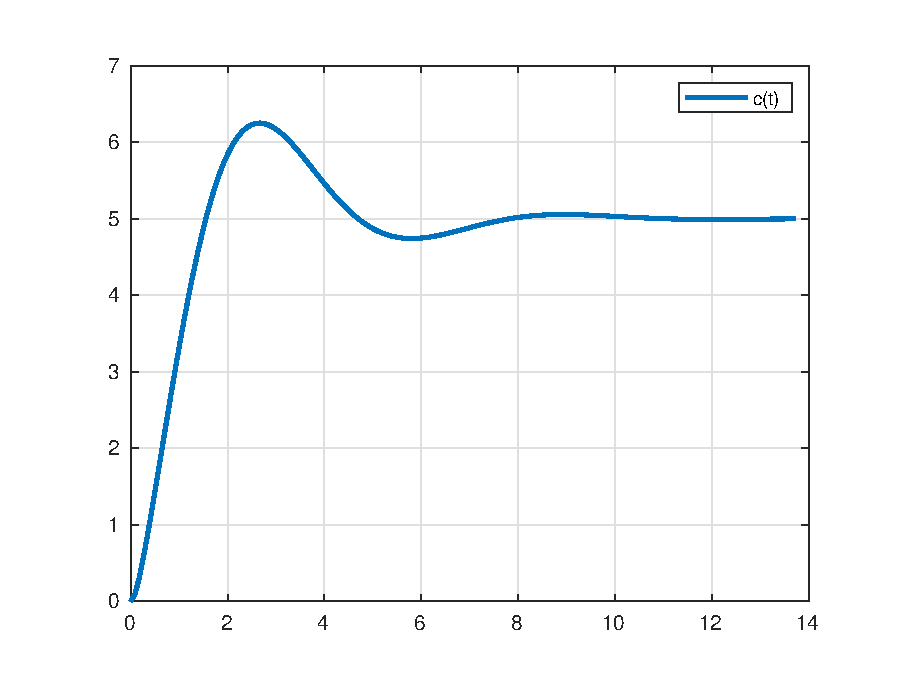
\includegraphics[width = 0.75\linewidth]{Figuras/ProblemasPI/Problema2/step.eps}
        \caption{Gráfico da resposta ao degrau do sistema}
        \label{fig:Q2A}                   
    \end{figure}

    Através do \mcode{stepinfo} verifica-se que o sobrevalor percentual é precisamente de 24,97\% e o tempo
    de subida de $T_r =1,13 \text{ s} $. 

\clearpage 
\newpage

\subsection*{b) }

    A Figura \ref{fig:LGR2Bsem} é o LGR do sistema sem o controlador. Através dela pode-se verificar que
    o sistema possui dois pólos puramente reais no semiplano esquerdo do domínio \textit{s}. Junto a isso,
    podemos ver que os pólos deslizam sobre o eixo real ao variar o ganho, até se encontrarem e 
    tornarem-se um par complexo.
    
    \begin{figure}[!ht]
        \centering
        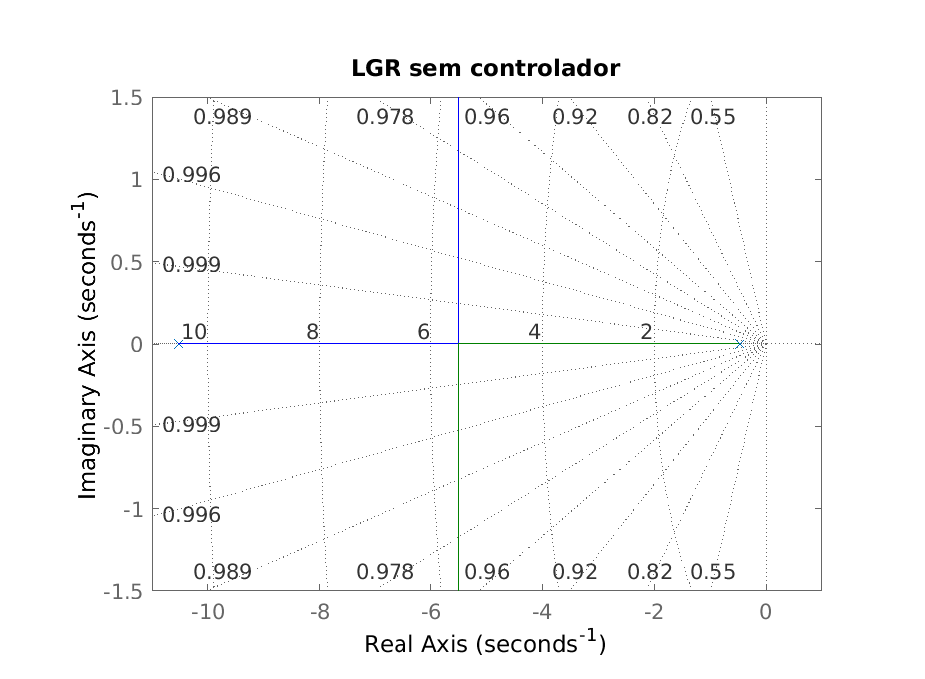
\includegraphics[width = 0.75\linewidth]{Figuras/ProblemasPI/Problema2/LGRsemcontrolador.eps}
        \caption{Lugar geométrico das raízes sem controlador}
        \label{fig:LGR2Bsem}                   
    \end{figure}

    Após adiconar o controlador o sistema tem o LGR apresentado na Figura \ref{fig:LGR2Bcom}
    
    \begin{figure}[!ht]
        \centering
        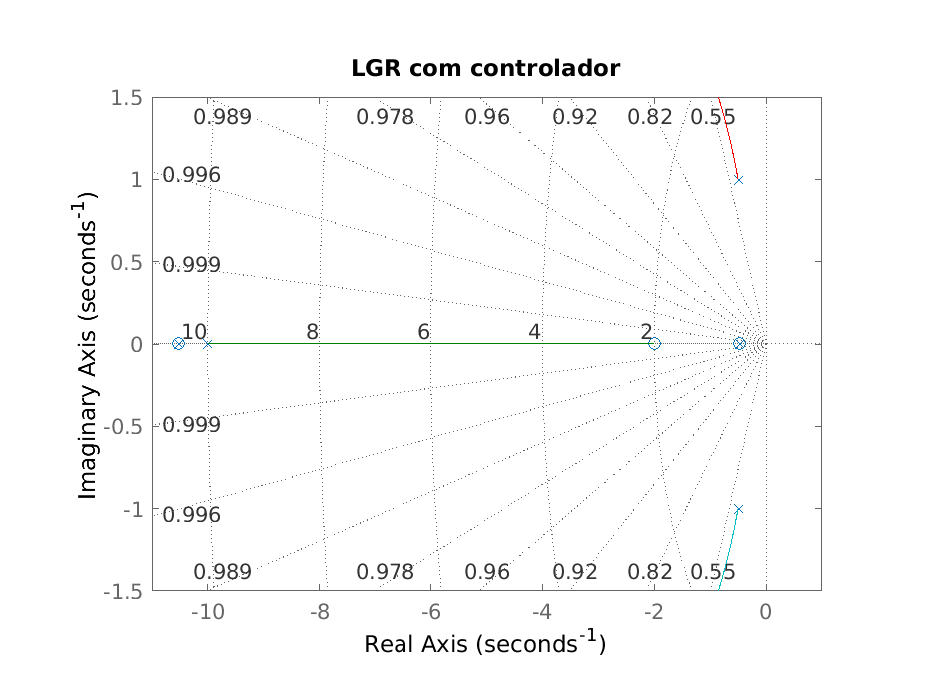
\includegraphics[width = 0.75\linewidth]{Figuras/ProblemasPI/Problema2/LGRcomcontrolador.eps}
        \caption{Lugar geométrico das raízes com controlador}
        \label{fig:LGR2Bcom}                   
    \end{figure}
\clearpage 
\newpage
 

\subsection*{c) }
    O tempo de amostragem foi determinado pelo tempo de subida divido por dez. 
    O sistema foi discretizado utilizando o segurador de ordem zero (ZoH). O Código \ref{Q2C} apresenta
    a discretização do modelo e a criação do gráfico da resposta do sistema a entrada degrau.
    
    \begin{lstlisting}[language=Matlab,label=Q2C,caption= Análise da estabilidade]
Ts = stepinfo(Gmf).RiseTime/10; %Tr = 1.1259
Gmfz = c2d(Gmf,Ts, 'zoh');
[yz,tz] = step(A*Gmfz); %salvando resultado do step

figure %fazendo uma figura para comparar
plot(t, y, 'LineWidth', 2)
hold on
stairs(tz, yz, 'LineWidth', 2);
hold off
legend('c(t)','c(kT)')
grid

%utilizando MAPE para avaliacao numerica
ape = abs((yz - y(1:length(yz)))/y(1:length(yz))); 
mape = mean(ape(isfinite(ape))); %retira o erro percentual do y=0
%mape = 4.7206e-04
    \end{lstlisting}

    O tempo de amostragem obtido foi de 113 ms. A FT em MF disceta é apresentada na equação \ref{eq:Gmfz2}
    A Figura \ref{fig:Stepctds2} apresenta a resposta dos sistema contínuo e discretizado sobrepostos. 

    \begin{equation}
        G_{mf}(z) = \frac{0.02922 z^2 - 0.002386 z - 0.01672}{z^3 - 2.203 z^2 + 1.503 z - 0.2898}
        \label{eq:Gmfz2}
    \end{equation}

    \begin{figure}[!ht]
        \centering
        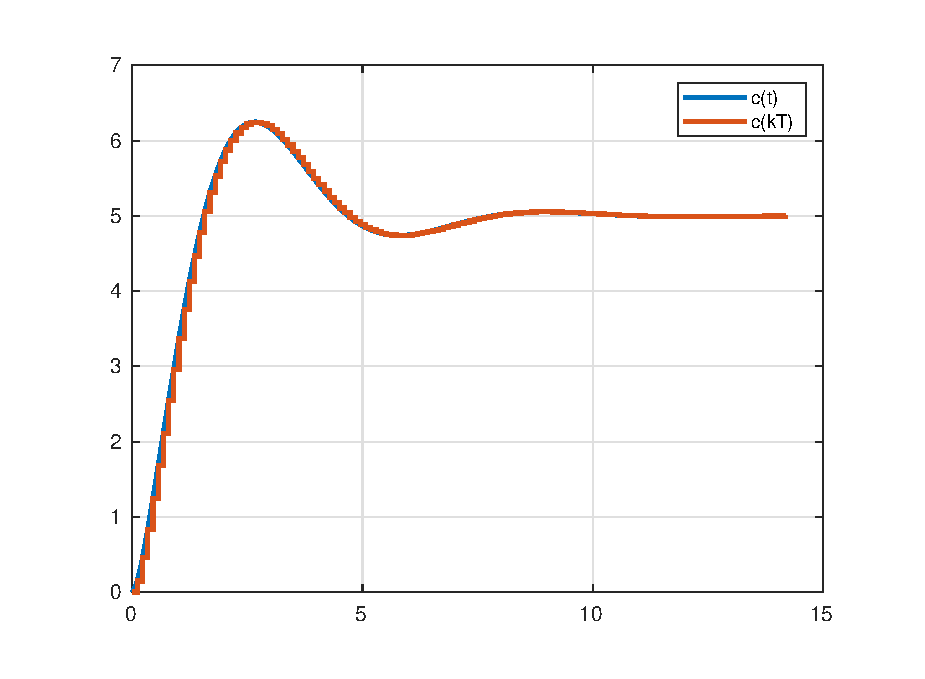
\includegraphics[width = 0.75\linewidth]{Figuras/ProblemasPI/Problema2/stepContinuoDiscreto.eps}
        \caption{Resposta ao degrau}
        \label{fig:Stepctds2}                   
    \end{figure}

    \subsubsection*{d)}

    O polinômio característico do sistema contínuo pode ser visto na equação \ref{eq:pcsc2}. A Tabela 
    \ref{tab:RE2} apresenta o desenvolvimento do método de Routh. 
    
    \begin{equation}
        Q(s) = s^3+11s^2+11.25s+12.5
        \label{eq:pcsc2}
    \end{equation}

    \begin{table}[!ht]
        \centering
        \vspace{0.5cm}
        \caption{Análise de estabilidade pelo método de Routh} 
        \begin{tabular}{r|lr}
            
            1 & 1 & 11.25 \\
            2 & 11 & 12.5 \\
            3 & 10.11\\
        \end{tabular}                
        \label{tab:RE2}
    \end{table}

    Verificamos que o sistema contínuo é estável.

    O polinômio característico do sistema discreto pode ser visto na equação \ref{eq:pcsd2}.

    \begin{equation}
        Q(z) = z^3 - 2.203 z^2 + 1.503 z - 0.2898
        \label{eq:pcsd2}
    \end{equation}

    A Tabela \ref{tab:JE2} apresenta o desenvolvimento do método de Jury para esse sistema.

    \begin{table}[!ht]
        \centering
        \caption{Análise de estabilidade pelo método de Jury} 
        \begin{tabular}{l| r r r r}
            & $z^0$ & $z^1$ & $z^2$ & $z^3$\\
            \hline
            1 & -0{,}2898 & 1{,}503 & -2{,}203 & 1\\
            2 & 1 & -2{,}203 & 1{,}503 & -0{,}2898\\
            3 & -0{,}8646 & 1{,}7674 & -0{,}916 & 0\\
        \end{tabular}                
        \label{tab:JE2}
    \end{table}

    Para verificar a estabilidade, como nosso polinômio é de ordem 3, devemos conferir os 4 critérios.

    - O primeiro critério: $Q(1)= 0,0102 \cdot 10^{-3} > 0$, satisfeito; \\
    - O segundo critério: $-1^3 Q(-1) = 4,9957 > 0$, satisfeito;\\
    - O terceiro critério: $|a_0| = 0,2898 < 1 = |a_3|$, satisfeito; \\
    - O quarto critério: $|b_0| = 0,916 > 0,8646 = |b_2| $, satisfeito. 
    
    Como o sistema discreto atende os quatro critérios de Jury necessários, é um sistema estável.

\newpage    
\subsection*{Problema 3:}

    O problema 3 pede para determinar um controlador proporcional para que o sistema torne-se estável. 
    A FT da planta é apresentado na equação \ref{eq:Gp3}.

    \begin{equation}
        G_p =  \frac{(s+20)}{s(s+10)^2}
        \label{eq:Gp3}
    \end{equation}

    Adicionando um controlador P, ou seja, $G_c = kp$, para controlar o sistema obtemos a FT de MF vista na equação
    \ref{eq:Gmf3}. 

    \begin{equation}
        T(s) = \frac{kp(s+20)}{s^3+20s^2+(100+kp)s+20kp}
        \label{eq:Gmf3}
    \end{equation}

    Foi visto no desenvolvimento que qualquer ganho, $kp > 0$, é o suficiente para manter o sistema
    estável. Como a questão não definiu um ganho, determinou-se livremente $kp = 2$.
    A questão pede então para obter o erro em regime estacionário para uma entrada degrau unitário
    e de uma rampa. 

\subsubsection*{a)}
    Para verificar a estabilidade foi observada a resposta do sistema a uma entrada a degrau que pode ser visto na Figura 
    \ref{fig:Q3A1}. Além disso também foi verificado a resposta do sistema a uma entrada rampa, como pode ser visto na Figura 
    \ref{fig:Q3A2}. Podemos ver que o erro em regime estacionário para uma entrada degrau é nulo e para uma entrada rampa é constante. 
    
    Analiticamente foi visto $e_{rampa}(\infty)=\frac{5}{kp}=2,5$. O script pode ser visto no bloco de código \ref{Q3A}. 

\begin{lstlisting}[language=Matlab,label=Q3A,caption=Análise da estabilidade]
% a)
nump = [1 20];
denp = [1 20 100 0];

Gp = tf(nump, denp);
Gc = 2;

Gma = Gc*Gp;
Gmf = Gma/(1+Gma);

[y,t] = step(Gmf);
figure
plot(t, y, 'LineWidth', 2);
legend('c(t)')
grid

s = tf('s');
[yr, tr] = step(Gmf/s); %entrada de rampa
figure
plot(tr, yr, 'LineWidth', 2);
hold on
plot(0:50,0:50,'LineWidth', 2);
legend('c(t)', 'r(t)')
hold off
axis([0 50 0 50])
grid    
\end{lstlisting}

\begin{figure}[!ht]
    \centering
    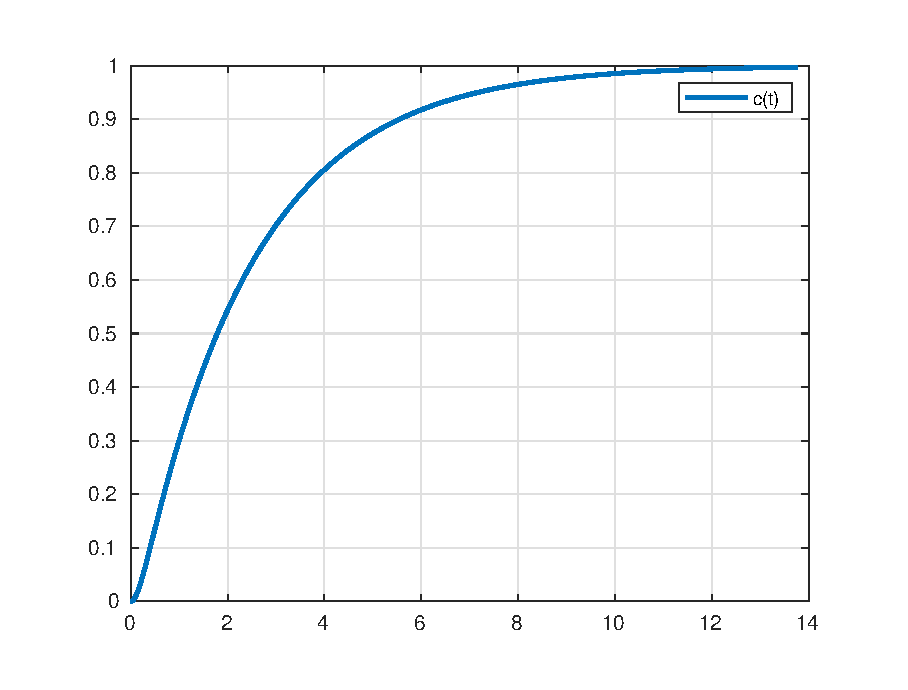
\includegraphics[width = 0.75\linewidth]{Figuras/ProblemasPI/Problema3/step.eps}
    \caption{Gráfico da resposta ao degrau do sistema}
    \label{fig:Q3A1}                   
\end{figure}

\begin{figure}[!ht]
    \centering
    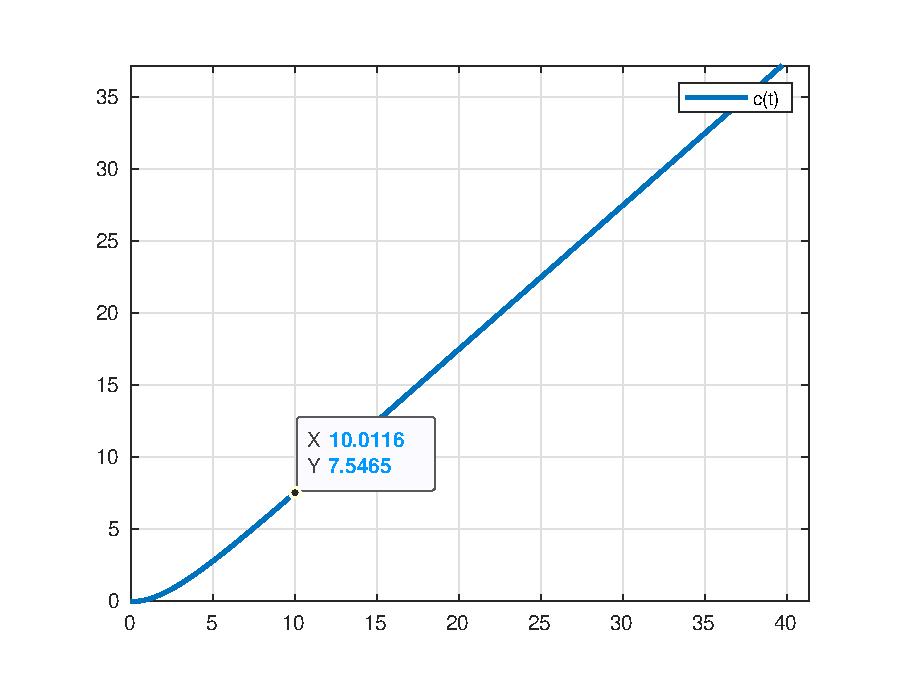
\includegraphics[width = 0.75\linewidth]{Figuras/ProblemasPI/Problema3/rampa.eps}
    \caption{Gráfico da resposta a uma rampa.}
    \label{fig:Q3A2}                   
\end{figure}

\newpage
\subsubsection*{b)}

    A Figura \ref{fig:LGR3Bsem} mostra o LGR do sistema sem controlador e a Figura \ref{fig:LGR3Bcom} o 
    LGR com controlador. Pode-se verificar que a realimentação removeu um polo e o ganho deslocou os polos 
    sobre o caminho traçado pelo LGR.


    \begin{figure}[!ht]
        \centering
        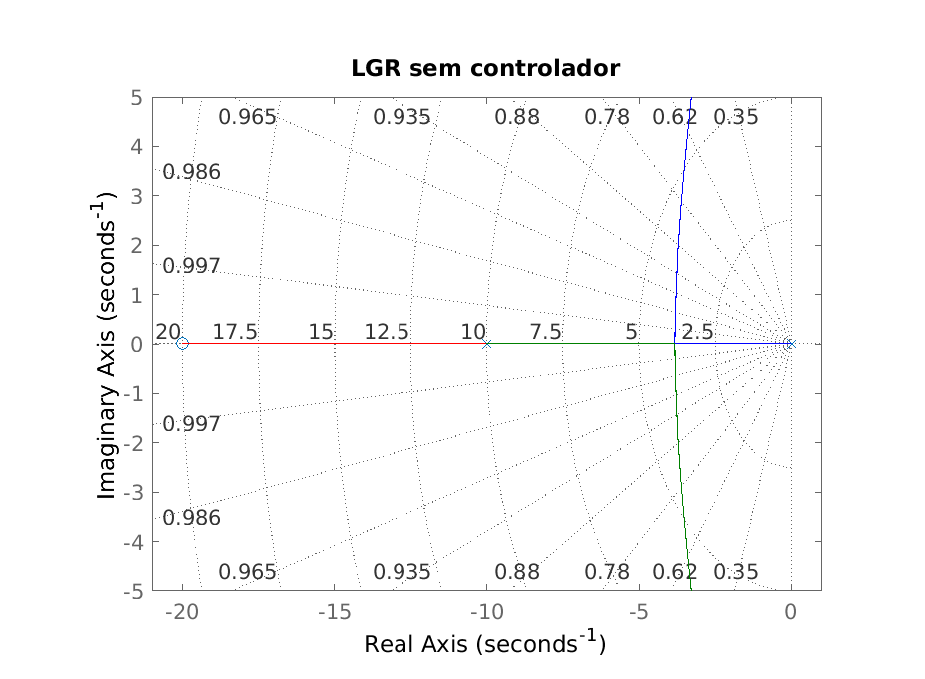
\includegraphics[width = 0.75\linewidth]{Figuras/ProblemasPI/Problema3/LGRsemControlador.eps}
        \caption{Lugar geométrico das raízes sem controlador.}
        \label{fig:LGR3Bsem}                   
    \end{figure}

    \begin{figure}[!ht]
        \centering
        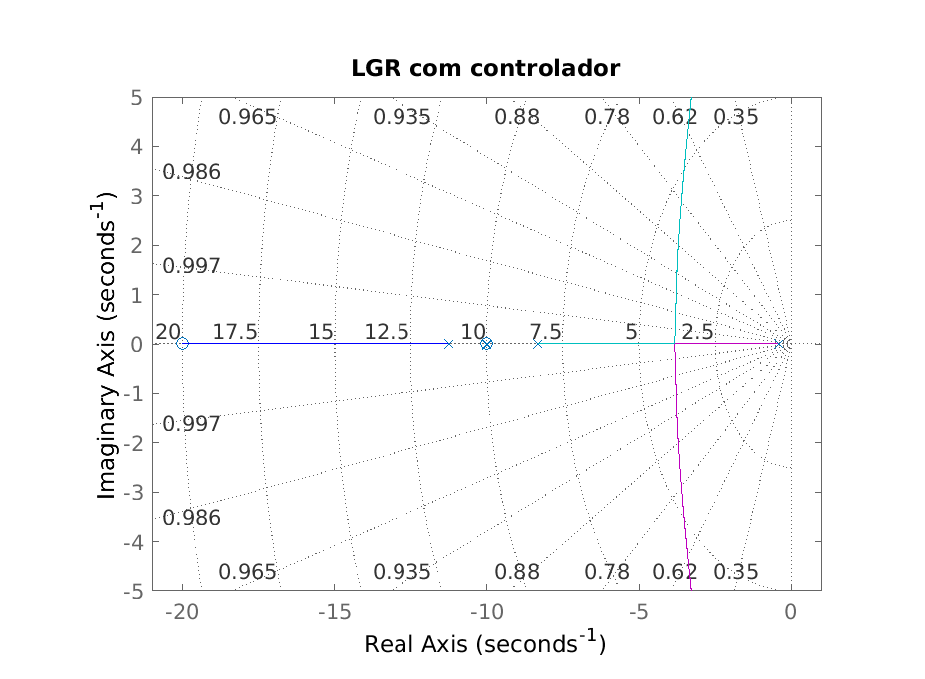
\includegraphics[width = 0.75\linewidth]{Figuras/ProblemasPI/Problema3/LGRcomControlador.eps}
        \caption{Lugar geométrico das raízes com controlador}
        \label{fig:LGR3Bcom}                   
    \end{figure}

    O bloco de código \ref{Q3B} apresenta o \textit{script} utilizado para obter os LGRs.

\begin{lstlisting}[language=Matlab,label=Q3B,caption= Análise da estabilidade]
        % b)
        % LGR sem controlador
        figure
        rlocus(Gp)
        axis([-21 1 -5 5])
        title('LGR sem controlador')
        grid
        % LGR com controlador
        figure
        rlocus(Gmf)
        axis([-21 1 -5 5])
        title('LGR com controlador')
        grid
 \end{lstlisting}


\newpage
\subsubsection*{c)}

    O tempo de amostragem foi determinado das mesma forma que anteriomente. O Código \ref{Q3C} apresenta
    a discretização do modelo e a criação do gráfico da resposta do sistema a entrada degrau.

    \begin{lstlisting}[language=Matlab,label=Q3C,caption=Análise da estabilidade]
Ts = stepinfo(Gmf).RiseTime/10; %Tr = 5.1535
Gmfz = c2d(Gmf, Ts, 'zoh');

[yz,tz] = step(Gmfz); %salvando resultado do step

figure %fazendo uma figura para comparar
plot(t, y, 'LineWidth', 2)
hold on
stairs(tz, yz, 'LineWidth', 2);
hold off
legend('c(t)','c(kT)')
grid

%utilizando MAPE para avaliacao numerica
ape = abs((yz - y(1:length(yz)))/y(1:length(yz))); 
mape = mean(ape(isfinite(ape))); %retira o erro percentual do y=0
%mape = 0.3376
    \end{lstlisting}

    O tempo de amostragem obtido foi de 515 ms. A FT em MF disceta é apresentada na equação \ref{eq:Gmfz3}
    A Figura \ref{fig:Stepctd3} apresenta a resposta dos sistema contínuo e discretizado sobrepostos. 

    \begin{equation}
        G_{mf}(z) = \frac{0.1411 z^4 + 0.05131 z^3 - 0.0003512 z^2 - 1.191e-06 z + 8.55e-09}{z^5 - 0.8307 z^4 + 0.02297 z^3 - 0.0002165 z^2 + 8.36e-07 z }
        \label{eq:Gmfz3}
    \end{equation}

    \begin{figure}[!ht]
        \centering
        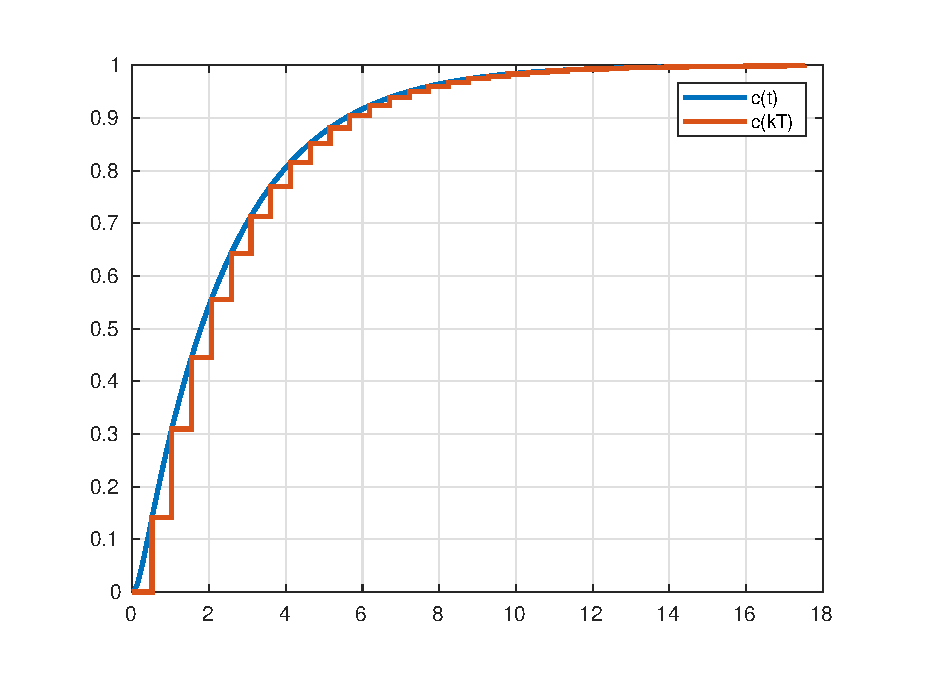
\includegraphics[width = 0.75\linewidth]{Figuras/ProblemasPI/Problema3/stepdiscreto.eps}
        \caption{Resposta ao degrau}
        \label{fig:Stepctd3}                   
    \end{figure}

    O MAPE do sistema discreto em relação ao sistema contínuo foi de $33,76 \cdot 10^{-2}$

\subsubsection*{d)}


    O polinômio característico do sistema contínuo pode ser visto na equação \ref{eq:pcsc3}. A Tabela 
    \ref{tab:RE3} apresenta o desenvolvimento do método de Routh. 

    \begin{equation}
        Q(s) = s^5 + 40 s^4 + 602 s^3 + 4080 s^2 + 1.1e04 s + 4000
        \label{eq:pcsc3}
    \end{equation}

    \begin{table}[!ht]
        \centering
        \vspace{0.5cm}
        \caption{Análise de estabilidade pelo método de Routh} 
        \begin{tabular}{r|lll}
            1 & 1 & 602 & 11.000 \\
            2 & 40 & 4080 & 4000 \\
            3 & 500 & 10.900 & 0\\
            4 & 4058 & 0 & 0
        \end{tabular}                
        \label{tab:RE3}
    \end{table}

    Verificamos que o sistema contínuo é estável.

    O polinômio característico do sistema discreto pode ser visto na equação \ref{eq:pcsd3}.

    \begin{equation}
        Q(z) = z^5 - 0.8307 z^4 + 0.02297 z^3 - 0.0002165 z^2 + 8.36e-07 z  - 1.115e-09                                                         
        \label{eq:pcsd3}
    \end{equation}

    A Tabela \ref{tab:JE3} apresenta o desenvolvimento do método de Jury para esse sistema.

    \begin{table}[!ht]
        \centering
        \caption{Análise de estabilidade pelo método de Jury} 
        \begin{tabular}{l| r r r r r r}
            & $z^0$ & $z^1$ & $z^2$ & $z^3$ & $z^4$ & $z^5$\\
            \hline
            1 & -1{,}115 & 8{,}36e-7 & -2{,}165e-4 & 2{,}297e-2 & -8{,}307e-1 & 0\\
            2 & -8{,}307e-1 & 2{,}297e-2 & -2{,}165e-4  & 8{,}36e-7 & -1{,}115 & 0\\
            3 & -8{,}35e-7 & 2{,}16e-4 & -2{,}3e-2  & 8{,}31e-1 & -1 & 0\\
            4 & -1 & 8{,}31e-1 & -2{,}3e-2  & 2{,}16e-4 & -8{,}35e-7 & 0\\
            5 & -2{,}15e-4 & -2{,}3e-2 & 8{,}31e-1  & -1 & 0 & 0\\
            6 & -1 &  8{,}31e-1  & -2{,}3e-2 & -2{,}15e-4 & 0 & 0\\
            7 & -2{,}28e-2 & 8{,}31e-1  & -1 & 0 & 0 & 0\\

        \end{tabular}                
        \label{tab:JE3}    
    \end{table}

    Para verificar a estabilidade, como nosso polinômio é de ordem 5, devemos conferir os 6 critérios.

    - O primeiro critério: $Q(1)= 0.192 > 0$, satisfeito; \\
    - O segundo critério: $-1^3 Q(-1) = 1.85 > 0$, satisfeito;\\
    - O terceiro critério: $|a_0| = 1.115e-9 < 1 = |a_5|$, satisfeito; \\
    - O quarto critério: $|b_0| = 1 >-8,35e-7 = |b_4| $, satisfeito. 
    - O quinto critério: $|c_0| = 1 > 2,15e-4 = |c_4| $, satisfeito. 
    - O sexto critério: $|d_0| = 0,916 > 0,8646 = |d_4| $, satisfeito. 
    
    Como o sistema discreto atende os seis critérios de Jury necessários, é um sistema estável.    

\newpage    
\subsection*{Problema 4:}

 O probleam 4 propõe achar um controlador proporcional que garanta que a constante de tempo em MF seja $\tau = 0.1\text{s}$ 
 e achar um controlador PI, para que o coef. de amortecimento seja $\zeta = 0,7$ e a frequência natural de oscilação 
 $\omega_0 = 114,2857 \text{rad/s}$. 

 Para o sistema utilizando o controlador P, os ganhos devem ser $kp = 0,08$ e $ki = 130,6122$ para que os 
 objetivos postos sejam cumpridos. A FT do sistema em MF pode ser visto na equação \ref{eq:Gp4P}.
   
 \begin{equation}
    T =  \frac{0,8}{s+10}
    \label{eq:Gp4P}
\end{equation}
 
 Para o sistema utilizando o controlador PI, os ganhos devem ser $kp = 1,58$ e $ki = 130,6122$ para que os 
 objetivos postos sejam cumpridos. A FT do sistema em MF pode ser visto na equação \ref{eq:Gp4PI}.

    \begin{equation}
        T =  \frac{10(1,58s+130,6122)}{s^2+160s+13061,22}
        \label{eq:Gp4PI}
    \end{equation}

No desenvolvimento analítico foi visto que o erro em regime estacionário para uma entrada degrau do sistema
com controlador P é $e(\infty) = 0,92$ e com controlador PI, $e(\infty) = 0$.
O código \ref{Q4A} apresenta o \textit{script} do Matlab para criar o Gráfico \ref{fig:Q4A}, que faz a comparação da resposta
dos dois sistemas.

\begin{lstlisting}[language=Matlab,label=Q4A,caption=Análise da estabilidade]
    % a)
    %FT da planta
    Gp = tf(10,[1 2]); 
    
    %Controlador Proporcional
    kp = 0.08;
    Gc = kp; %Ganho do controlador
    Gmap = Gc*Gp; %Malha Aberta
    Gmfp = Gmap/(1+10*Gmap); %Malha fechada
    
    %Controlador PI
    kp = 1.58; 
    ki = 130.6122;
    Gmapi = tf(10*[kp ki], [1 2 0]);
    Gmfpi = Gmapi/(1+Gmapi);
    
    % a)
    
    %step para avaliar a resp do sistema
    [yp,tp] = step(Gmfp, 0.6);
    [ypi, tpi] = step(Gmfpi, 0.6);
    
    %graficos comparativos
    figure
    plot(tp, yp, 'LineWidth', 2);
    hold on
    plot(tpi, ypi, 'LineWidth', 2);
    hold off
    legend('P', 'PI')
    grid
\end{lstlisting}

\begin{figure}[!ht]
    \centering
    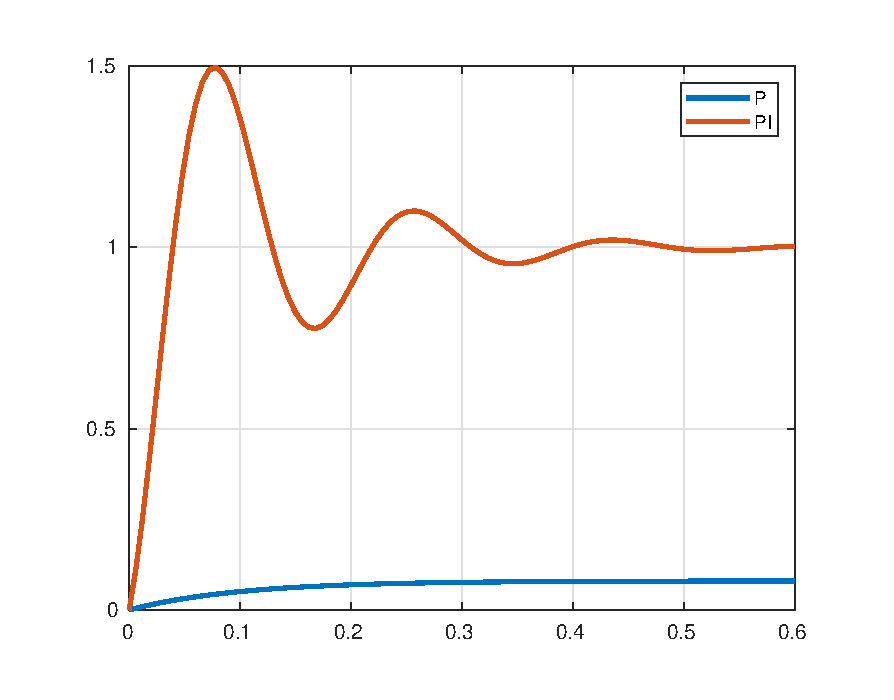
\includegraphics[width = 0.75\linewidth]{Figuras/ProblemasPI/Problema4/step.eps}
    \caption{Gráfico da resposta ao degrau do sistema utilizando um controlador P e um PI.}
    \label{fig:Q4A}                   
\end{figure}

Vemos que o sobrevalor foi de $50\%$ ao utilizar o controlador PI e que esse foi o único controle que em regime permitiu
um erro nulo.

\subsubsection*{b)}

    A Figura \ref{fig:LGR4Bsem} mostra o LGR do sistema sem controlador, a Figura \ref{fig:LGR4BP} o 
    LGR com controlador P e a Figura \ref{fig:LGR4BPI}  o LGR com controlador PI. 


    \begin{figure}[!ht]
        \centering
        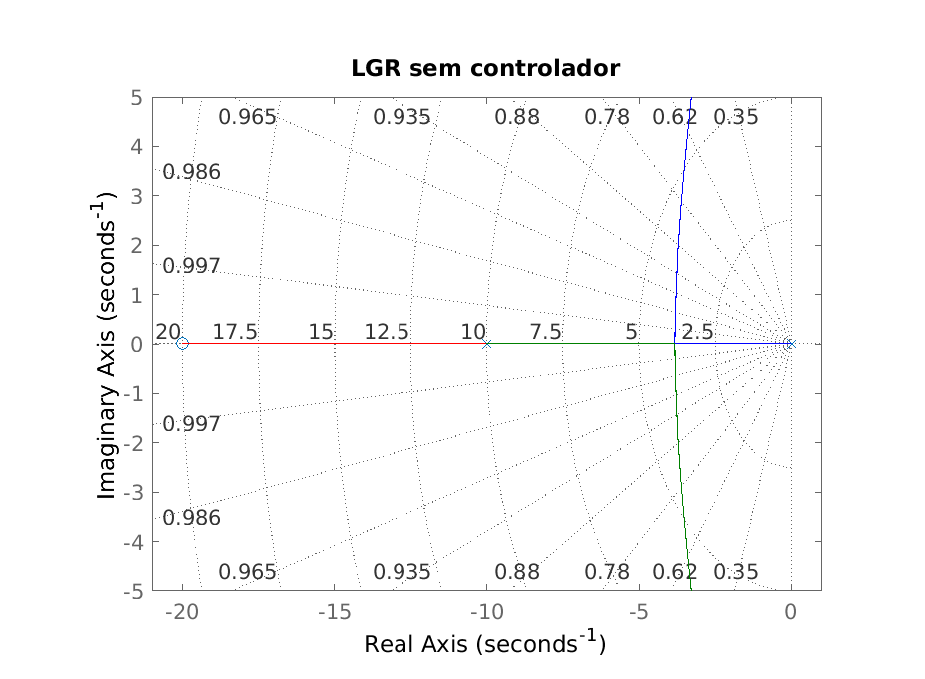
\includegraphics[width = 0.75\linewidth]{Figuras/ProblemasPI/Problema3/LGRsemControlador.eps}
        \caption{Lugar geométrico das raízes sem controlador.}
        \label{fig:LGR4Bsem}                   
    \end{figure}

    \begin{figure}[!ht]
        \centering
        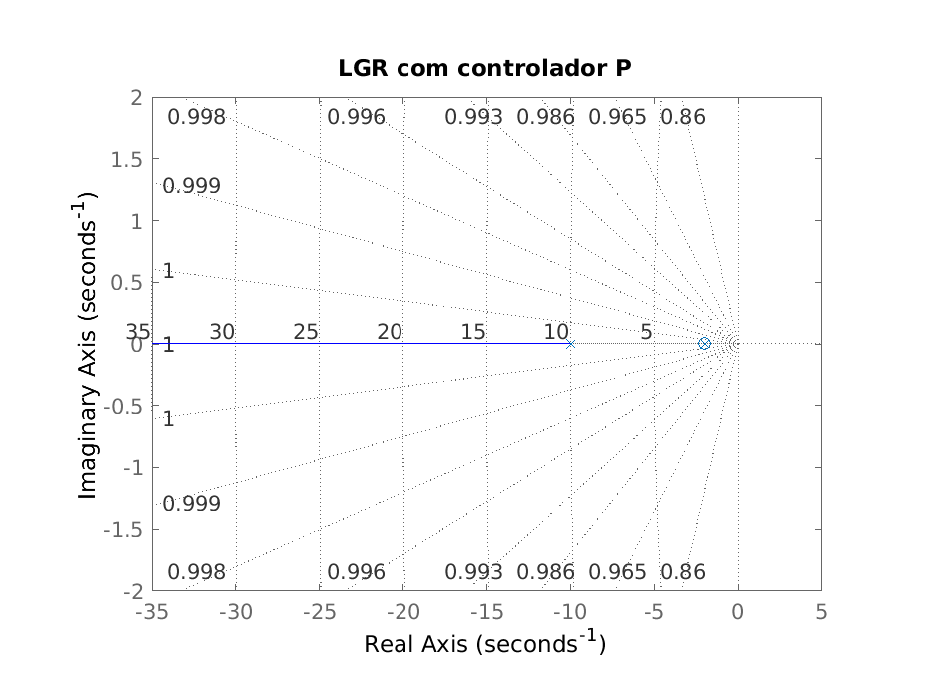
\includegraphics[width = 0.75\linewidth]{Figuras/ProblemasPI/Problema4/lgrcomP.eps}
        \caption{Lugar geométrico das raízes com controlador P}
        \label{fig:LGR4BP}                   
    \end{figure}

    \begin{figure}[!ht]
        \centering
        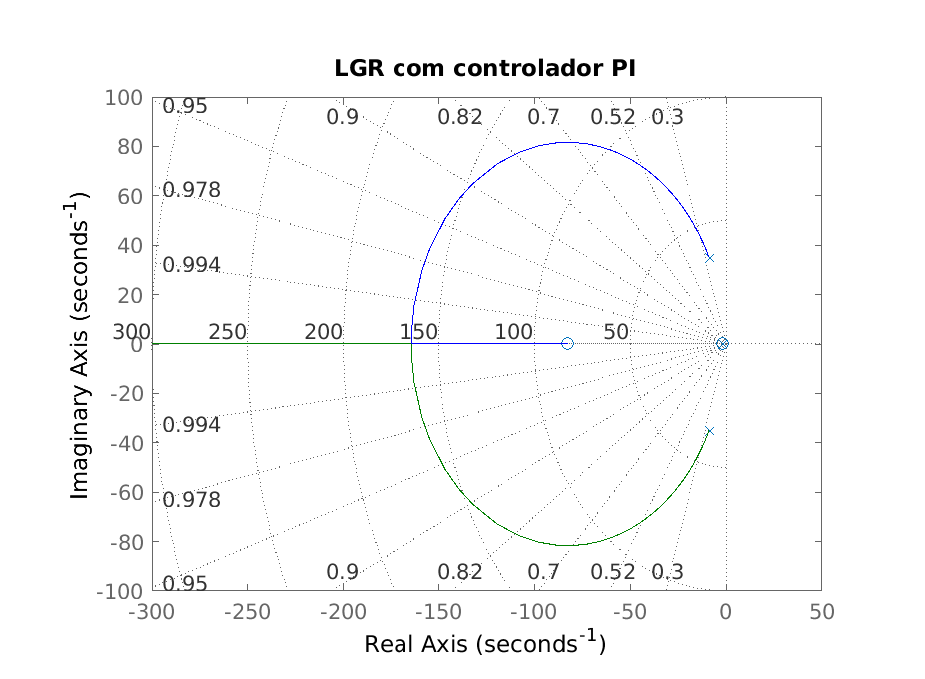
\includegraphics[width = 0.75\linewidth]{Figuras/ProblemasPI/Problema4/lgrcomPI.eps}
        \caption{Lugar geométrico das raízes com controlador PI}
        \label{fig:LGR4BPI}                   
    \end{figure}

    Pode-se verificar que o controlador P, Figura \ref{fig:LGR4BP}, é suficiente para tornar o sistema estável, 
    porém mantém um único polo que desliza (ao alterar o ganho) pelo eixo real, não permitindo a redução do
    erro. O controlador PI, Figura \ref{fig:LGR4BPI}, adiciona um polo e torna-o em um conjugado complexo. A alteração 
    do ângulo da reta que passa pelo polo e pela origem representa a alteração no amortecimento.

\clearpage 
\newpage
\subsubsection*{c)}
    O tempo de amostragem foi de 22ms para o sistema com controlador P e de 3ms para o com controlador PI.
    O Código \ref{Q3C} apresenta a discretização do modelo e a criação do gráfico da resposta dos sistemas 
    a entrada degrau.

\begin{lstlisting}[language=Matlab,label=Q4C,caption= Análise da estabilidade]
Tsp = stepinfo(Gmfp).RiseTime/10; %Tr = 5.1535
Tspi = stepinfo(Gmfpi).RiseTime/10;
Gmfpz = c2d(Gmfp, Tsp, 'zoh');
Gmfpiz = c2d(Gmfpi, Tspi, 'zoh');

%salvando resultado do step
[yzp,tzp] = step(Gmfpz, 0.6); 
[yzpi,tzpi] = step(Gmfpiz, 0.6);

%avaliando o controlador P
figure 
plot(tp, yp, 'LineWidth', 2)
hold on
stairs(tzp, yzp, 'LineWidth', 2);
hold off
legend('c(t)','c(kT)')
title('Resposta ao degrau Controlador P')
grid

%utilizando MAPE para avaliacao numerica
ape = abs((yzp - yp(1:length(yzp)))/yp(1:length(yzp))); 
mapep = mean(ape(isfinite(ape))); %retira o erro percentual do y=0
%mape = 0.0142
\end{lstlisting}

A FT em MF disceta do sistema com controlador P é apresentada na equação \ref{eq:Gmfz4P} e a do sistema controlador PI \ref{eq:Gmfz4PI}.
A Figura \ref{fig:Stepctds4P} apresenta a resposta do sistema contínuo e discretizado com controlador P, e a Figura \ref{fig:Stepctds4PI}
com controlador PI.

\begin{equation}
    G_{mf}(z) = \frac{0.01578}{z - 0.8028}
    \label{eq:Gmfz4P}
\end{equation}

\begin{equation}
    G_{mf}(z) = \frac{0.05192 z - 0.04045}{z^2 - 1.936 z + 0.9479}
    \label{eq:Gmfz4PI}
\end{equation}

\begin{figure}[!ht]
    \centering
    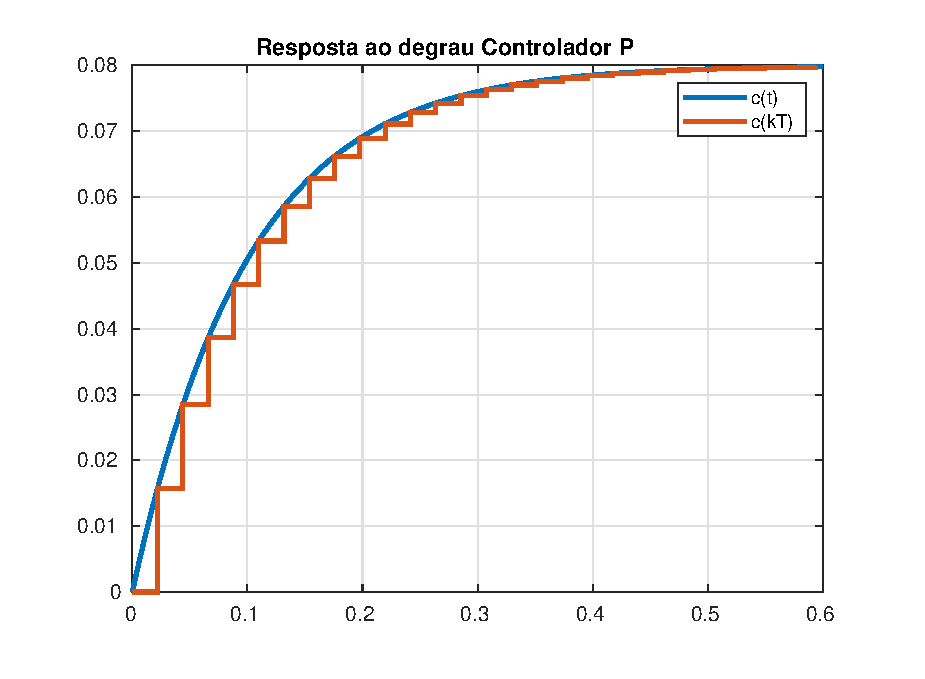
\includegraphics[width = 0.75\linewidth]{Figuras/ProblemasPI/Problema4/stepPz.eps}
    \caption{Resposta ao degrau}
    \label{fig:Stepctds4P}                   
\end{figure}

\begin{figure}[!ht]
    \centering
    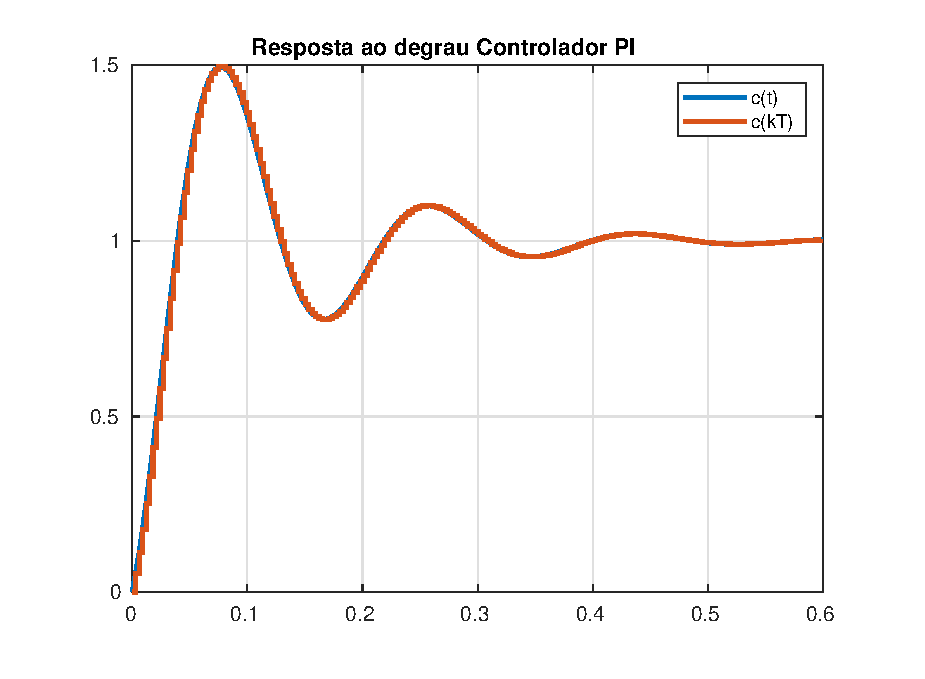
\includegraphics[width = 0.75\linewidth]{Figuras/ProblemasPI/Problema4/stepPIz.eps}
    \caption{Resposta ao degrau}
    \label{fig:Stepctds4PI}                   
\end{figure}

O MAPE do sistema discreto em relação ao contínuo com controlador P foi de $1,42 \cdot 10^{-2}$ \%  e
com o controlador PI foi de $ 0,15 \cdot 10^{-2}$ \% .

\clearpage 
\newpage
\subsubsection*{d)}


Os polinômios característicos do sistema contínuo com controlador P e PI, podem ser vistos, respectivamente
através das equações \ref{eq:pcsc4P} e \ref{eq:pcsc4PI}.

\begin{equation}
    Q(s) = s+10
    \label{eq:pcsc4P}
\end{equation}

\begin{equation}
    Q(s) = s^2 + 17,8 s + 1306
    \label{eq:pcsc4PI}
\end{equation}

O sistema com controlador P é facilmente verificado como
estável dado que possui um único polo real negativo. A Tabela \ref{tab:RE4} apresenta o desenvolvimento do método de
Routh para verificar a estabilidade do sistema com controlador PI. 

\begin{table}[!ht]
    \centering
    \vspace{0.5cm}
    \caption{Análise de estabilidade pelo método de Routh} 
    \begin{tabular}{r|ll}
        1 & 1 & 1306 \\
        2 & 17,8 & 0 \\
        3 & 1306 & 0 \\
    \end{tabular}                
    \label{tab:RE4}
\end{table}

Verificamos que o sistema contínuo é estável.
Os polinômios característicos dos sistemas discretos com controlador P e PI, podem ser vistos nas equações
\ref{eq:pcsd4P} e \ref{eq:pcsd4PI}, respectivamente.

\begin{equation}
    Q(z) = z - 0.8028                                                          
    \label{eq:pcsd4P}
\end{equation}

\begin{equation}
    Q(z) = z^2 - 1.936 z +  0.9479                                                       
    \label{eq:pcsd4PI}
\end{equation}

Podemos ver que o sistema discreto do controlador P, equação \ref{eq:pcsc4P} é estável pois $|z|<1$. Já para o 
sistema com o controlador PI é de ordem 2, então é necessário verificar três critérios, sem necessidade de tabela.

- O primeiro critério: $Q(1)= 0.0119 > 0$, satisfeito; \\
- O segundo critério: $-1^3 Q(-1) = 3.88 > 0$, satisfeito;\\
- O terceiro critério: $|a_0| = 0.9479 < 1 = |a_2|$, satisfeito.

Como o sistema atende os três critérios de Jury necessários, é um sistema estável. 

\subsection*{Problema 5:}

O problema 5 pede para determinar as caracteristicas do sistema com FT em MA da equação \ref{eq:Gma5}.

\begin{equation}
    G_{ma} =  \frac{25}{s(s+6)}
    \label{eq:Gma5}
\end{equation}

Esse sistema possui um tempo de assentamento $Ts = 1.33s$. A partir disso, a questão pede para criar um
compensador para diminui-lo. O ganho do compensador encontrado é visto na equação \ref{eq:compensador}

\begin{equation}
    G_c = s + 18.75
    \label{eq:compensador}
\end{equation}

Com a adição do compensador a FT em MF foi a vista na equação \ref{eq:Gmf5}

\begin{equation}
    G_{mf} =  \frac{25 s + 468.8}{s^2 + 31 s + 468.8}
    \label{eq:Gmf5}
\end{equation}

\subsubsection*{a)}
Para verificar a estabilidade foi observada a resposta do sistema a uma entrada a degrau que pode ser visto na Figura 
\ref{fig:Q5A}. O bloco de código \ref{Q5A} apresenta o código para construção do gráfico.

\begin{lstlisting}[language=Matlab,label=Q5A,caption=Análise da estabilidade]
%step para avaliar a resp do sistema
[y,t] = step(Gmf,0.35);

%avaliando o controlador P
figure 
plot(t, y, 'LineWidth', 2)
legend('c(t)')
title('Resposta ao degrau')
grid
\end{lstlisting}

\begin{figure}[!ht]
    \centering
    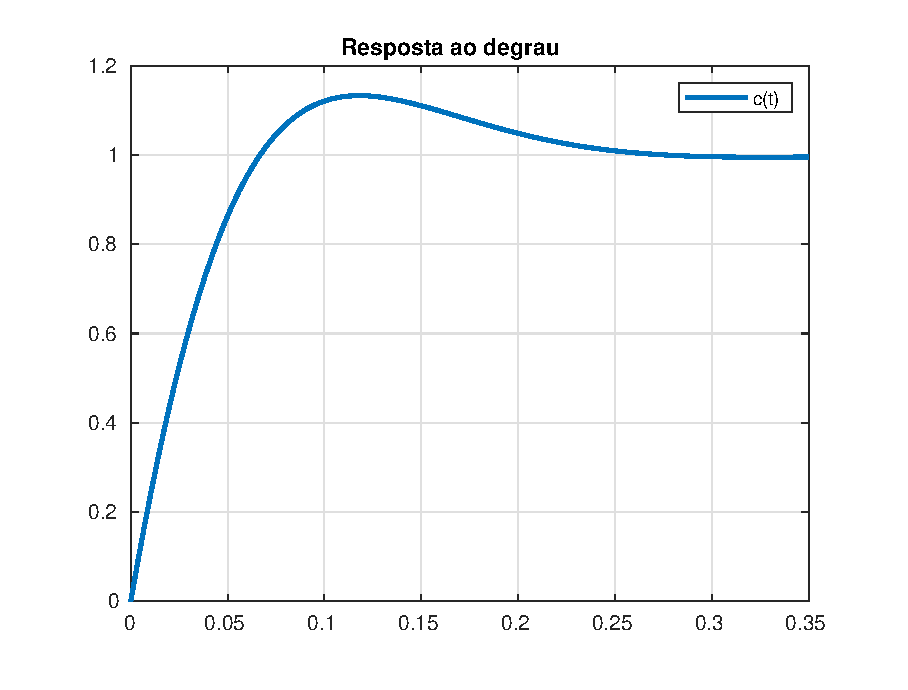
\includegraphics[width = 0.75\linewidth]{Figuras/ProblemasPI/Problema5/step.eps}
    \caption{Resposta ao degrau}
    \label{fig:Q5A}                   
\end{figure}


\clearpage
\newpage
\subsubsection*{b)}
A Figura \ref{fig:LGR5Bsem} é o LGR do sistema sem o compensador e a Figura \ref{fig:LGR5Bcom} o LGR com o 
compensador.

\begin{figure}[!ht]
    \centering
    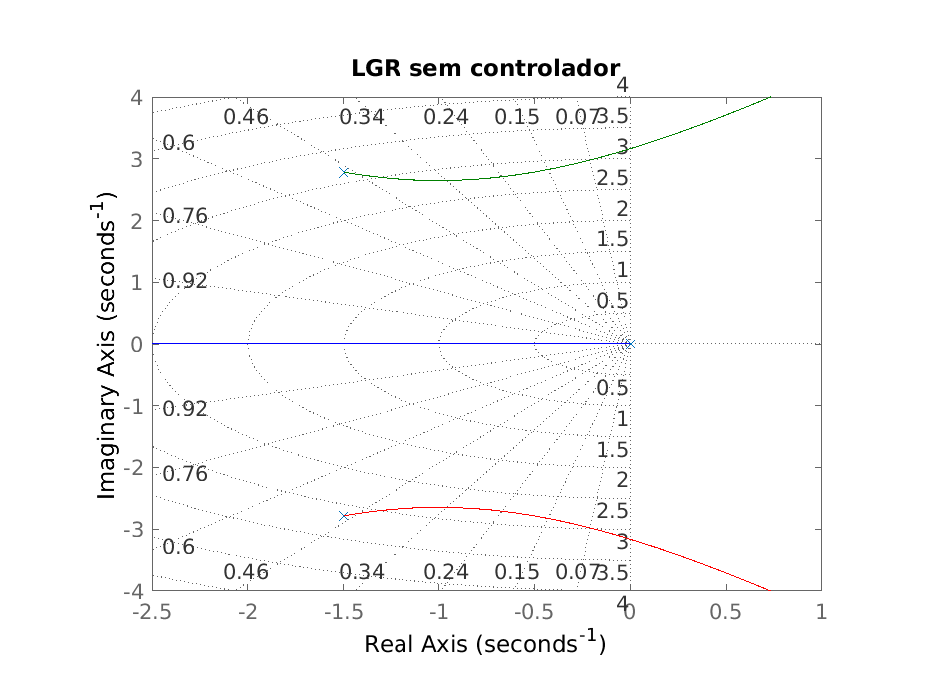
\includegraphics[width = 0.75\linewidth]{Figuras/ProblemasPI/Problema1/LGRsemControlador.eps}
    \caption{Lugar geométrico das raízes sem controlador}
    \label{fig:LGR5Bsem}                   
\end{figure}

\begin{figure}[!ht]
    \centering
    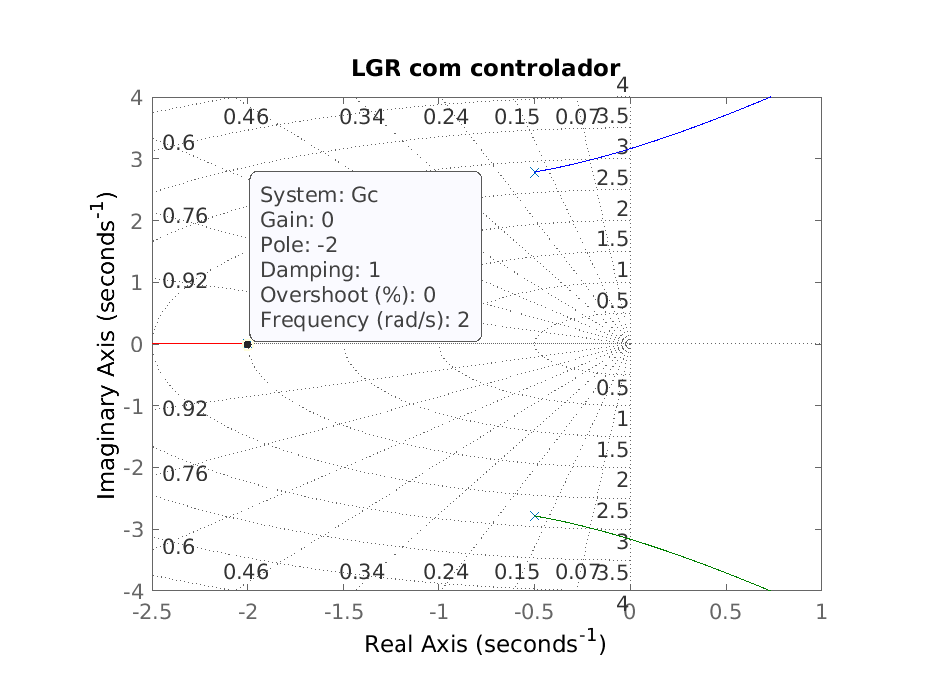
\includegraphics[width = 0.75\linewidth]{Figuras/ProblemasPI/Problema1/LGRcomControlador.eps}
    \caption{Lugar geométrico das raízes com controlador}
    \label{fig:LGR5Bcom}                   
\end{figure}

O compensador moveu os polos de forma a ficarem mais negativos. 

\subsubsection*{c)}

O Código \ref{Q5C} apresenta a discretização do modelo e a criação do Gráfico \ref{fig:Stepctds5} da resposta do sistema a entrada degrau.

\begin{lstlisting}[language=Matlab,label=Q5C,caption=Análise da estabilidade]
% c)
Ts = stepinfo(Gmf).RiseTime/10; %Tr = 0.05
Gmfz = c2d(Gmf, Ts, 'zoh');

%salvando resultado do step
[yz,tz] = step(Gmfz); 

%avaliando o controlador P
figure 
plot(t, y, 'LineWidth', 2)
hold on
stairs(tz, yz, 'LineWidth', 2);
hold off
legend('c(t)','c(kT)')
title('Resposta ao degrau')
grid

%utilizando MAPE para avaliacao numerica
ape = abs((yz - y(1:length(yz)))/y(1:length(yz))); 
mape = mean(ape(isfinite(ape))); %retira o erro percentual do y=0
%mape = 9.3241e-04
\end{lstlisting}


\begin{figure}[!ht]
    \centering
    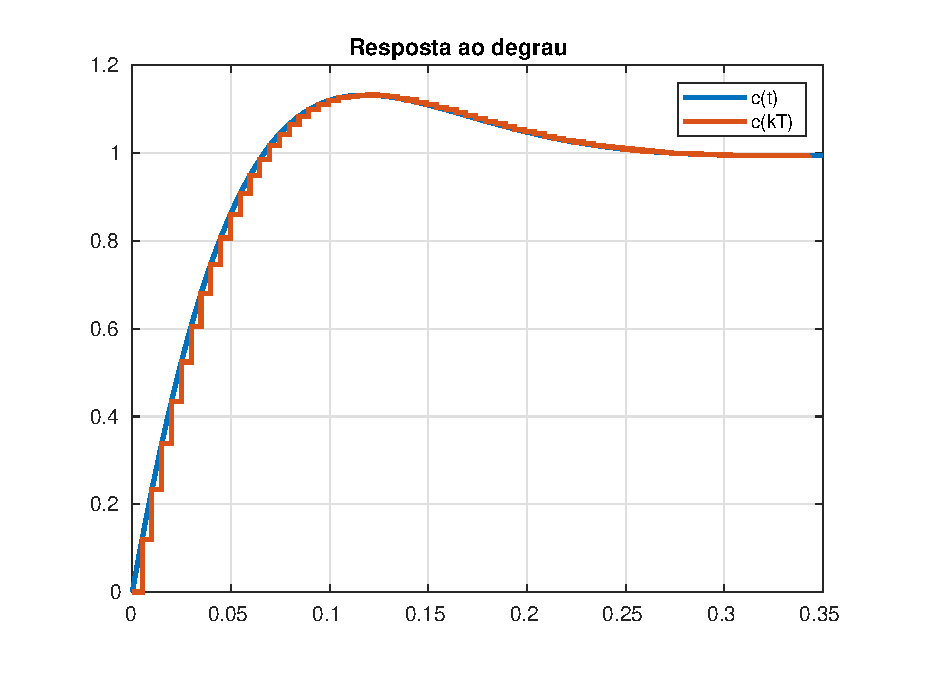
\includegraphics[width = 0.75\linewidth]{Figuras/ProblemasPI/Problema5/stepz.eps}
    \caption{Resposta ao degrau}
    \label{fig:Stepctds5}                   
\end{figure}

O tempo de discretização foi $Ts = 5ms$. O MAPE foi de $9,32 \cdot 10^{-2}$ \%. A função de transferência do sistema discreto pode ser vista através
da equação \ref{eq:Gmfz5}. 

\begin{equation}
    G_{mf}(z) = \frac{ 0.1204 z - 0.1097}{ z^2 - 1.846 z + 0.8572}
    \label{eq:Gmfz5}
\end{equation}


\newpage
\subsubsection*{d)}

O polinômio característico do sistema contínuo pode ser visto na equação \ref{eq:pcsc5}.

\begin{equation}
    Q(s) = s^2 + 31 s + 468.8
    \label{eq:pcsc5}
\end{equation}

A Tabela \ref{tab:RE5} apresenta o desenvolvimento do método de Routh para verificar a estabilidade do sistema.
\begin{table}[!ht]
    \centering
    \vspace{0.5cm}
    \caption{Análise de estabilidade pelo método de Routh} 
    \begin{tabular}{r|ll}
        1 & 1 & 468{,}8 \\
        2 &  31 & 0 \\
        3 & 14532.8 & 0 \\
    \end{tabular}                
    \label{tab:RE5}
\end{table}

Verificamos que o sistema contínuo é estável.
O polinômio característico do sistema discreto pode ser visto na equação \ref{eq:pcsd5}.

\begin{equation}
    Q(z) =  z^2 - 1.846 z + 0.8572                                                        
    \label{eq:pcsd5}
\end{equation}

Como deve-se obsevar somente as três prime pois o sistema é de ordem 2, não necessita-se da tabela.

- O primeiro critério: $Q(1)= 0.0112 > 0$, satisfeito; \\
- O segundo critério: $-1^3 Q(-1) = 3.7032 > 0$, satisfeito;\\
- O terceiro critério: $|a_0| = 0.8572  < 1 = |a_2|$, satisfeito.

O sistema discreto é, então, estável. 